Implementemos el siguiente sistema en Simulink:

\begin{figure}[ht!]
    \begin{center}
    \resizebox{0.95\linewidth}{!}{%
        \begin{tikzpicture}[
            font=\sffamily,
            bloque/.style={
                draw=black,
                fill=white,
                line width=0.65pt,
                inner sep=0pt,
                outer sep=0pt,
            },
            conexion/.style={
                line width=0.45pt,
                -{Triangle[length=2.2mm,width=2mm]}
            }
        ]

            %-----------------------------------------
            % Bloques de entrada.
            %-----------------------------------------
            \node[
                bloque,
                minimum size=0.8cm
            ] (escalon) at (0,0) {};

            \node[
                bloque,
                minimum size=0.8cm
            ] (senal) at (2.6,-2.2) {};

            %-----------------------------------------
            % Sumador con dos entradas positivas.
            %-----------------------------------------
            \node[
                bloque,
                circle,
                minimum size=5.4mm
            ] (suma) at (2.6,0) {};

            \node[inner sep=0pt, font=\scriptsize]
                at ([xshift=-1.3mm]suma.center) {$+$};

            \node[inner sep=0pt, font=\scriptsize]
                at ([yshift=-1.3mm]suma.center) {$+$};

            %-----------------------------------------
            % Funcion de transferencia.
            %-----------------------------------------
            \node[
                bloque,
                minimum width=6cm,
                minimum height=2.2cm,
                font={\normalsize\boldmath}
            ] (G) at (8,0)
                {$\displaystyle
                    \frac{a}{b\cdot s^3+c\cdot s^2+d\cdot s+e}
                $};

            %-----------------------------------------
            % Scope y puerto de salida.
            %-----------------------------------------
            \node[
                bloque,
                minimum width=0.8cm,
                minimum height=0.84cm
            ] (scope) at (14.4,0) {};

            \node[
                bloque,
                rounded corners=1.9mm,
                minimum width=0.8cm,
                minimum height=0.38cm,
                font={\sffamily\normalsize}
            ] (salida) at (14.4,1.95) {1};

            %-----------------------------------------
            % Icono de la entrada escalon.
            %-----------------------------------------
            \begin{scope}[shift={(escalon.center)}]
                \draw[line width=0.55pt]
                    (-0.32,-0.26) -- (0,-0.26)
                    -- (0,0.27) -- (0.31,0.27);
            \end{scope}

            %-----------------------------------------
            % Icono del generador de senal.
            %-----------------------------------------
            \begin{scope}[shift={(senal.center)}]

                % Pequenos ejes interiores.
                \draw[gray!65, line width=0.45pt]
                    (-0.25,-0.30) -- (-0.25,0.30)
                    (-0.30,-0.24) -- (0.31,-0.24);

                % Forma de la senal.
                \draw[
                    line width=0.55pt,
                    line join=round
                ]
                    (-0.21,-0.02) -- (-0.13,-0.02)
                    -- (-0.09,-0.05) -- (-0.06,-0.18)
                    -- (-0.01,0.30) -- (0.07,0.24)
                    -- (0.13,-0.13) -- (0.17,0.28)
                    -- (0.22,-0.23) -- (0.29,-0.25);

            \end{scope}

            %-----------------------------------------
            % Pantalla dentro del Scope.
            %-----------------------------------------
            \begin{scope}[shift={(scope.center)}]
                \draw[
                    line width=0.65pt,
                    rounded corners=1.4pt
                ]
                    (-0.29,-0.06) rectangle (0.29,0.30);
            \end{scope}

            %-----------------------------------------
            % Conexiones de entrada.
            %-----------------------------------------
            \draw[conexion]
                (escalon.east) -- (suma.west);

            \draw[conexion]
                (senal.north) -- (suma.south);

            \draw[conexion]
                (suma.east) -- (G.west);

            %-----------------------------------------
            % Salida bifurcada.
            %-----------------------------------------
            \coordinate (derivacion) at (12.55,0);

            % Camino horizontal hasta el Scope.
            \draw[conexion]
                (G.east) -- (scope.west);

            % Rama superior hacia el puerto 1.
            \draw[conexion]
                (derivacion) |- (salida.west);

            % Punto negro de la bifurcacion.
            \fill (derivacion) circle[radius=1.65pt];

        \end{tikzpicture}%
    }
\end{center}
\end{figure}



\noindent donde 

\begin{align*}
    a &= 1000 + 1100\ \text{rand}\\
    b &= \text{round(rand)}\\
    c &= 40 + 5\ \text{rand}\\
    d &= 100 + 50\ \text{rand}\\
    e &= 1000 + 200\ \text{rand}\\
\end{align*}

\noindent son los parámetros de la función transferencia.

La siguiente figura representa la salida para el sistema

\begin{figure}[ht!]
    \centering
    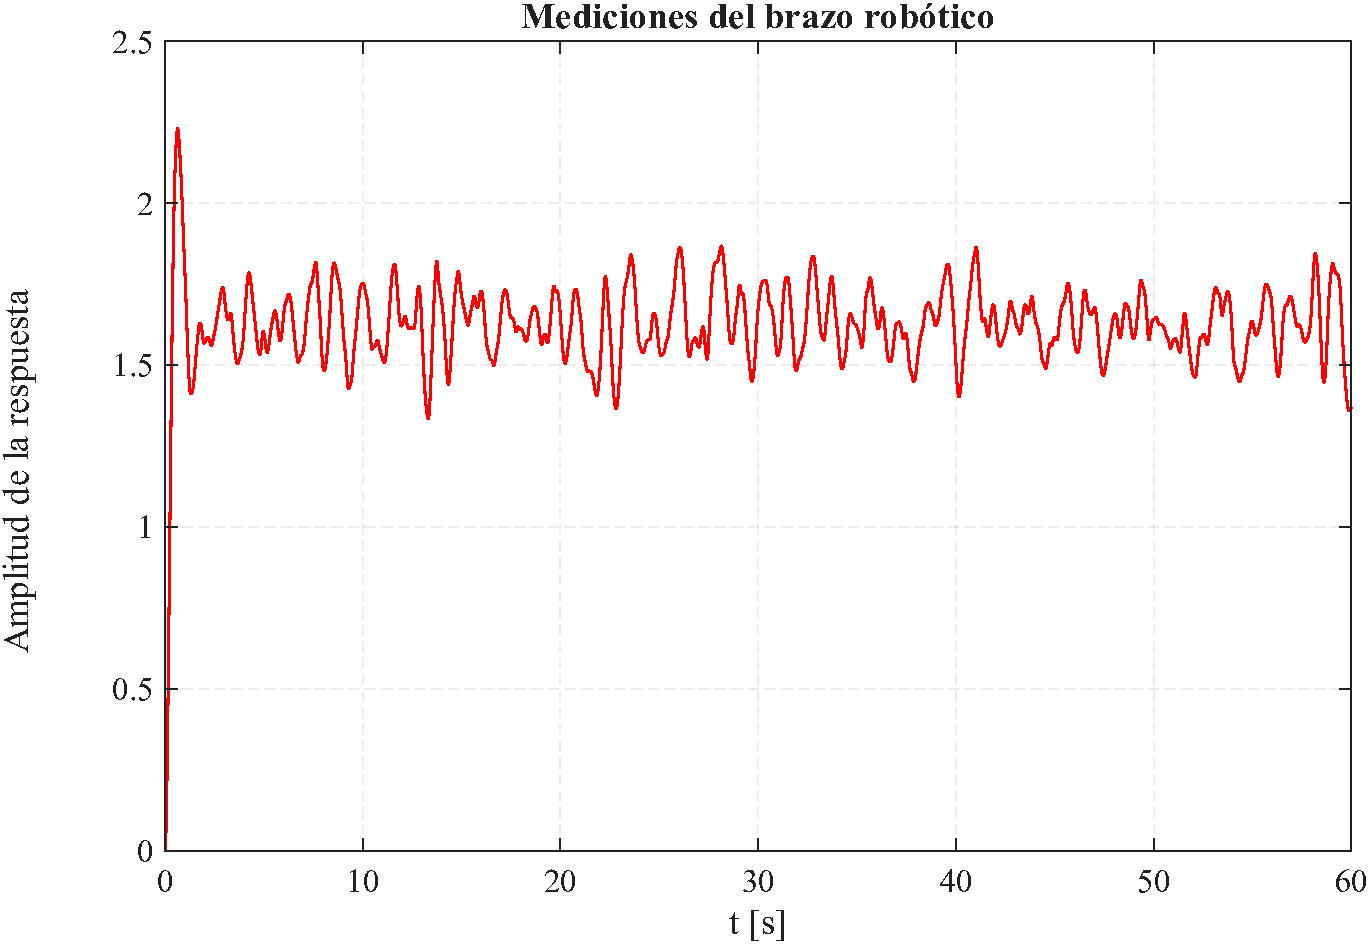
\includegraphics[width=0.8\textwidth]{imagenes/brazo_robotico.pdf}
    \caption{Respuesta del brazo robótico ante una entrada escalón}
    \label{fig:3}
\end{figure}    



Dado que no conocemos nuestro sistema podemos suponer que es un sistema de segundo orden:

\begin{equation}
    G(s) = k\ \frac{\omega^2}{s^2 + 2\zeta\omega + \omega^2}
\end{equation}


\noindent donde 


\begin{align}
    k &= \frac{\displaystyle\sum_{i = n-49}^{n} y_i}{50}\\
    \zeta &= \sqrt{\frac{-2\log\left(\displaystyle\frac{y_{\text{máx}}}{k} - 1\right)}{\pi^2 -2\log\left(\displaystyle\frac{y_{\text{máx}}}{k} - 1\right)}}\\
    \omega &= \frac{1.1 + 0.125\zeta + 0.469\zeta^2}{t_d} 
\end{align}


El tiempo de retardo, $t_d$, es el tiempo que tarda el sistema para llegar a la mitad de su valor final. El siguiente código de MATLAB muestra cómo calcular este valor, implementado el sistema $G(s)$:

\begin{lstlisting}
%Disminuimos el ruido tomando los ultimos 50 valores
n = length(y);
k = sum(y(n - 49:end)/50);

function zeta = factor_amortiguamiento(y, k)
    ymax = max(y);
    num = -2*log(ymax/k - 1);
    den = pi^2 - 2*log(ymax/k - 1);
    zeta = sqrt(num/den);
end

%Factor de amortiguamiento
zeta = factor_amortiguamiento(y, k);
indice = find(y > 0.5*k, 1, 'first');
%Calculo del tiempo de retardo
td = t(indice);
%frecuencia natural del sistema
omega = (1.1 + 0.125*zeta + 0.469*zeta^2)/td;

%Armamos la funciin transferencia de segundo orden
G = tf([k*omega^2], [1, 2*omega*zeta, omega^2]);

[yout, tout] = step(G);


subplot(2,1,1)
plot(t, y, 'r')
hold on
step(G, 'm')
subplot(2,1,2)
plot(t(1:400), y(1:400), 'r')
hold on 
plot(tout, yout, 'm')

\end{lstlisting}


La figura \ref{fig:4} representa la respuesta del modelo ante el sistema real. Por último, veamos el sistema cuando éste no presenta ruido, esto es \texttt{sis\_no\_ruido = tf([a], [b, c, d, e]);}. En la figura \ref{fig:5} se observa distintos diagramas que representan a los dos sistemas. Se observa que los polos de ambos son prácticamente iguales.

\newpage

\begin{figure}[ht!]
    \centering
    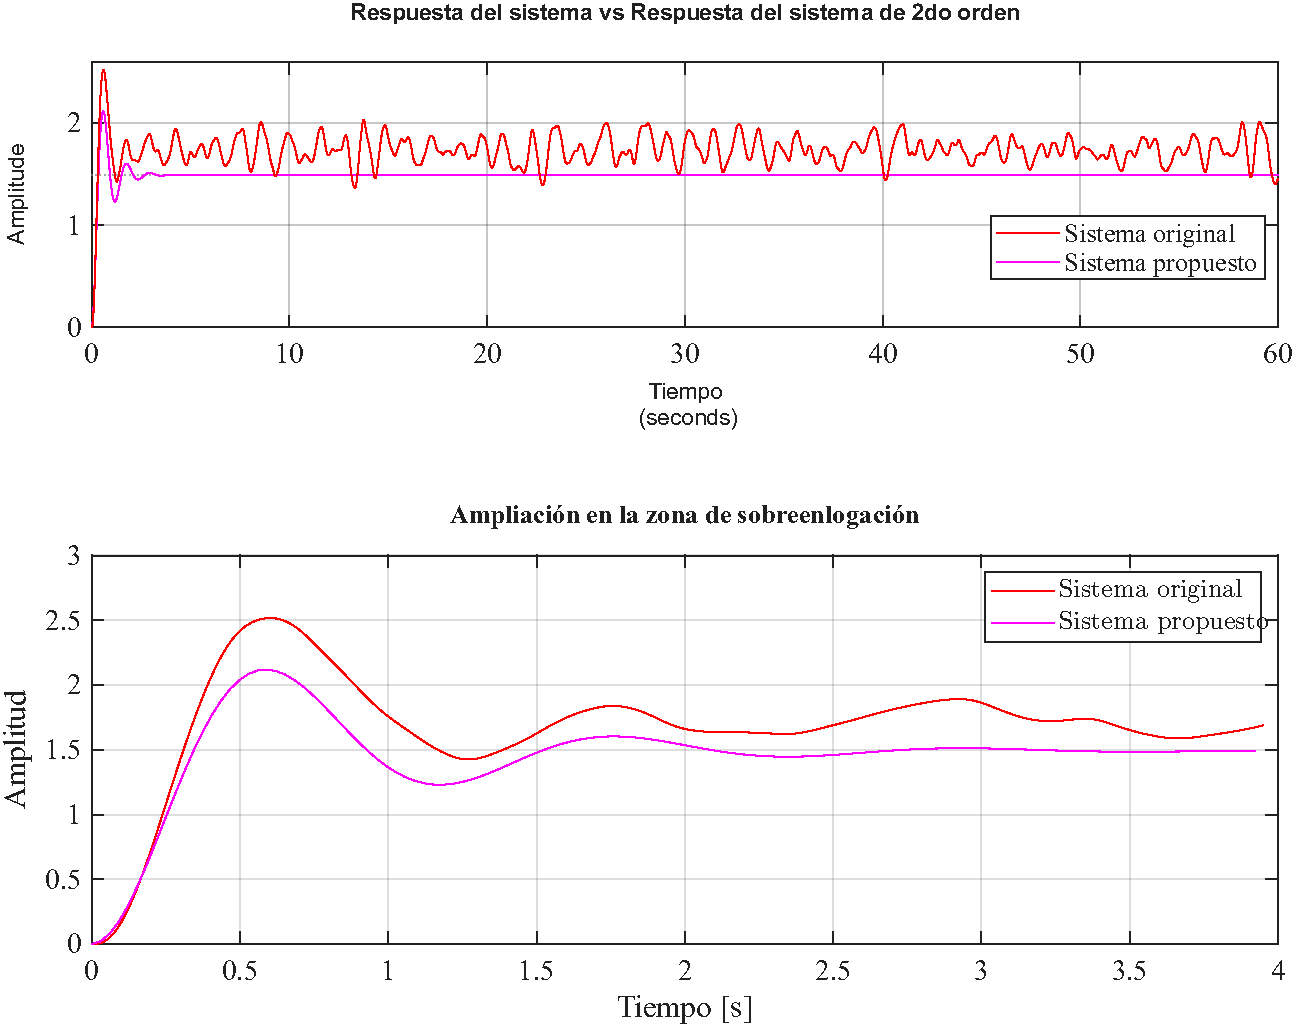
\includegraphics[width=0.9\textwidth]{imagenes/comparacion_respuestas.pdf}
    \caption{Respuestas del modelo propuesto vs el sistema que representa el movimiento del robot.}
    \label{fig:4}
\end{figure}


\begin{figure}[ht!]
    \centering
    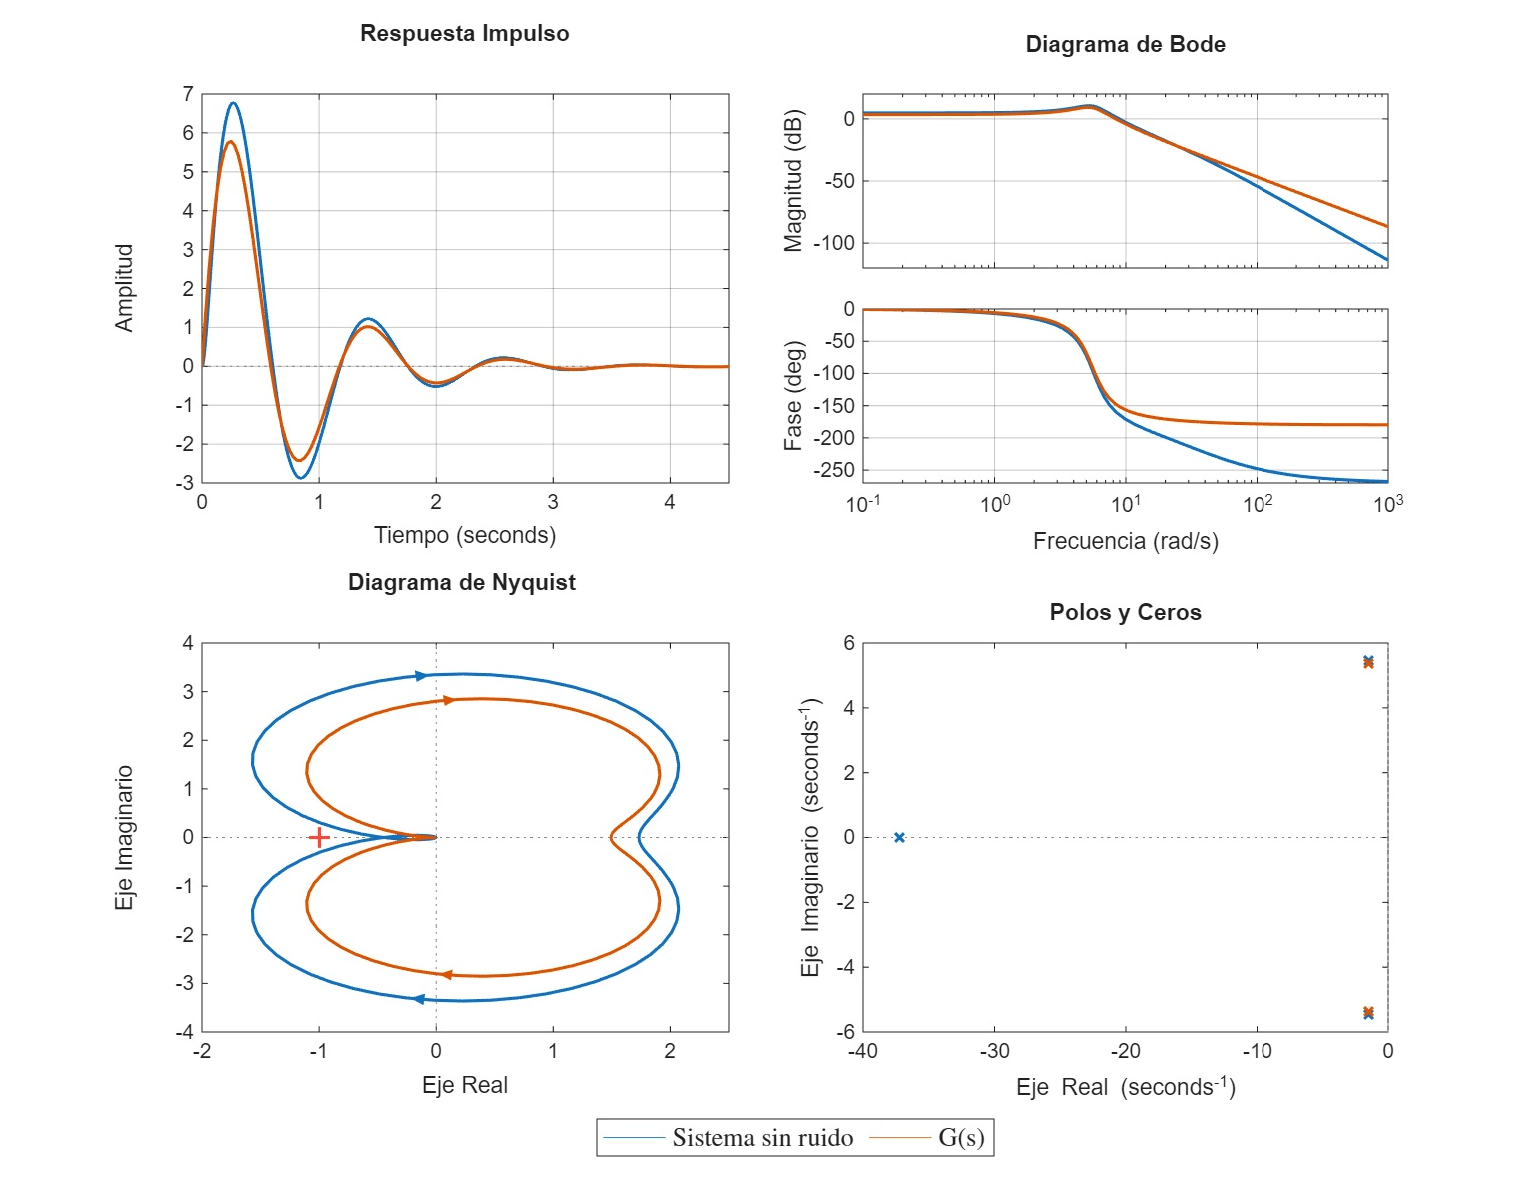
\includegraphics[width=0.9\textwidth]{imagenes/Linear System Analyzer Responses.pdf}
    \caption{Comparación del sistema sin ruido con respecto al sistema propuesto de segundo orden.}
    \label{fig:5}
\end{figure}


\newpage

En la figura \ref{fig:6} se compara algunos tiempos ante la entrada escalón


\begin{figure}[ht!]
    \centering
    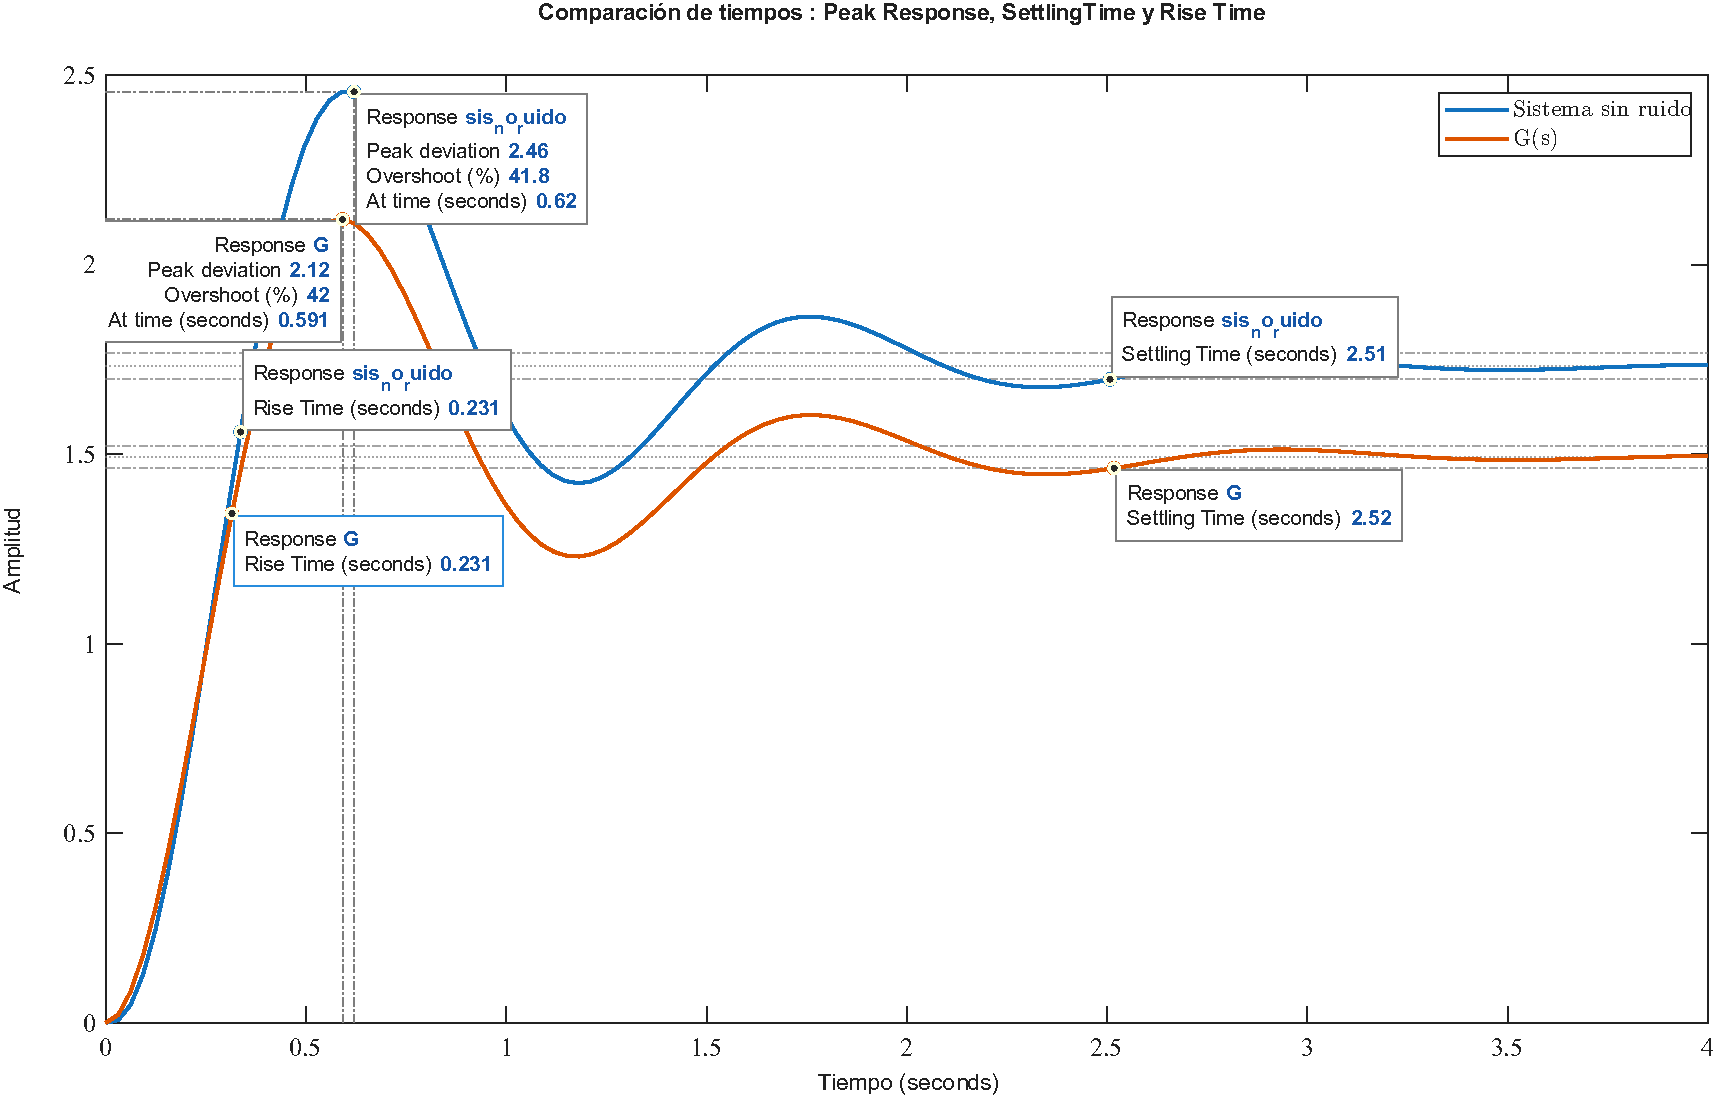
\includegraphics[width=\textwidth]{imagenes/Analisis de tiempos.pdf}
    \caption{Algunas características de los sistemas ante la entrada escalón.}
    \label{fig:6}
\end{figure}



Por último, se mencionan algunos errores que se cometen al momento de estimar la función de transferencia $G(s)$:

\begin{enumerate}
    \item El orden del sistema o modelo.
    \item Utilizar datos pocos fiables.
    \item Estimar mal sus parámetros. 
    \item Validarlo de manera inadecuada: concluir que el modelo representa una buena estimicación al sistema original.
\end{enumerate}